\chapter{Herramientas utilizadas}
\label{cap:capitulo3}

El desarrollo de los dos nuevos ejercicios de Robotics Academy han abarcado varios campos: programación, Docker, modelado y simulación de robots, ROS y ROS2, visión artificial, machine learning, desarrollo web... por lo que es necesario introducir y describir las herramientas y tecnologías utilizadas.\\



\section{Lenguajes de programación}
\label{sec:lenguajes_programacion}


% -- SUBSECCIÓN C++
% ----------------
\subsection{C++}
\label{subsec:c++}

C++ \cite{c++} es un lenguaje de programación diseñado en 1979 por Bjarne Stroustrup. Deriva del lenguaje C, y destaca principalmente porque incorpora el paradigma de la \textit{Programación Orientada a Objetos} (POO). Además, incorpora una novedosa librería que facilita el desarrollo de Software de calidad: \textit{STL} (Standard Template Library): vector, stack, map, etc. Desde sus comienzos, C++ ha tenido varias versiones que han incorporado nuevas características al lenguaje (98, 11, 14, 17...) siendo C++20 la última.\\

\begin{code}[H]
\begin{lstlisting}[language=C++]
#include <iostream>

int main(int argc, char ** argv)
{
	std::cout << "Hello World!\n";
	return 0;
}
\end{lstlisting}
\caption[Hola mundo en C++]{Hola mundo en C++}
\label{cod:holamundo_cplusplus}
\end{code}

¿Cuál ha sido la utilidad de C++ en este proyecto? La programación de un \textit{plugin} que permite mover a una persona simulada en simulador Gazebo con el teclado (versión C++17).\\




% -- SECCIÓN PYTHON
% -------------------
\subsection{Python}
\label{subsec:python}

Python \cite{python_doc} es un lenguaje de programación \textit{interpretado} \footnote{\textbf{Interprete} (programación): programa informático que se encarga de ejecutar las instrucciones de otro programa sin compilación previa} que destaca por su legibilidad, facilidad y soportabilidad con el paradigma \textit{POO}. Posee características particulares que lo diferencian de otros lenguajes de programación como puede ser el uso estricto de indentación en bloques de código, o incluso la capacidad de crear listas mezcladas de diferentes tipos de datos. Las versión más reciente de Python es la 3.10.\\

\begin{code}[H]
\begin{lstlisting}[language=Python]
print("Hola mundo")
\end{lstlisting}
\caption[Hola mundo en Python]{Hola mundo en Python}
\label{cod:holamundo_python}
\end{code}

¿Cuál ha sido la utilidad de Python en este proyecto? El desarrollo de la infraestructura interna que da soporte a los dos nuevos ejercicios de Robotics Academy, programación de nodos de ROS (más en la sección \ref{sec:ros}) y ficheros de lanzamiento, creación de los módulos HAL y GUI y desarollo de las soluciones de referencia de los ejercicios (versión Python 3.8)\\




% -- SECCION ROS
% ----------------
\section{ROS (Robot Operating System)}
\label{sec:ros}
ROS (Robot Operating System) \cite{ROS} es un \textit{middleware} \footnote{\textbf{Middleware}: software que se sitúa entre las aplicaciones y el sistema operativo} que ayuda a la programación de robots a través de varias librerías y herramientas desarrolladas por la comunidad de software libre. Entre las ayudas que proporciona este entorno/ecosistema están la abstracción del hardware, controladores de dispositivos, herramientas de visualización (rviz) y geometría espacial (transformadas, tfs) entre otros. ROS está mantenido por la fundación OpenRobotics.\\

El \textit{funcionamiento} de ROS se basa en una arquitectura \textit{cliente-servidor} centralizado donde un nodo principal se encarga del intercambio de mensajes entre otros nodos que forman la aplicación (remotos o locales), los cuales se comportan como \textit{publicadores o suscriptores} del proceso de comunicación. El objetivo es dividir el software robótico en secciones o \textit{nodos} que se encargan de realizar tareas específicas de manera concurrente: recogida de datos de la cámara, ejecución de una máquina de estados o árboles de comportamiento (Behavior Trees), recogida de las lecturas del láser, navegación, etc.\\

El intercambio de mensajes se realiza a través \textit{topics}. Un nodo puede tener publicadores, suscriptores o ambos. Cuando un nodo publica un mensaje lo hace a través de un \textit{topic} que gestiona el nodo maestro. Si otro nodo quiere leer ese mensaje tendrá que suscribirse al \textit{topic} correspondiente. Por ejemplo: en nuestro robot Turtlebot2 podemos comandar velocidades enviando mensajes de tipo geometry\_msgs.msg.Twist a través del \textit{topic} /cmd\_vel. En la figura se puede ver con más detalle \ref{fig:ros_master_comunicacion}\\

\begin{figure} [H]
  \begin{center}
    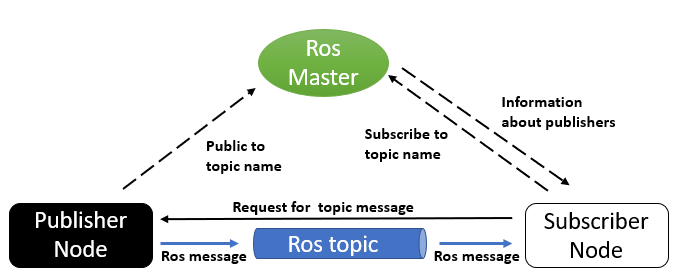
\includegraphics[width=15cm]{imagenes/cap3/ros_master_communication.png}
  \end{center}
  \caption{Comunicación del nodo Master con los nodos Intermedios (ROS)}
  \label{fig:ros_master_comunicación}
\end{figure}\

Desde un principio, ROS se ha ejecutado sobre sistemas operativos de tipo Linux, aunque han ido surgiendo versiones beta para otros SOs como Windows o MacOS X. La primera distribución de ROS salió en 2010 (ROS Box Turtle) y a partir de ahí han ido surgiendo nuevas distribuciones siendo la actual y estable ROS Noetic.\\

Las librerías que incorpora ROS están desarrolladas en \textit{C++} y \textit{Python}. Con estos lenguajes de programación podemos desarrollar los nodos de los paquetes que tendrá nuestra aplicación. También incorpora un conjunto de comandos de \textit{Shell} \footnote{\textbf{Shell}: Programa que toma entradas del usuario a través del teclado y pasa esos comandos al sistema operativo para realizar una función específica} para realizar tareas de depuración, creación, compilación, etc.\\

En 2016 surge ROS2, nuevo ecosistema basado en ROS que incorpora nuevas mejoras como la calidad de servicio, los \textit{lifecycle nodes}, o seguridad mediante DDS para asegurar la autenticación de los nodos y la integridad de los mensajes. Al igual que con ROS ha tenido varias distribuciones siendo la primera \textit{ROS Ardent}. La versión más reciente y estable es \textit{ROS Foxy}, que es la que hemos usado en este proyecto.\\

¿Cuál ha sido la utilidad de ROS2 en este proyecto?
\begin{itemize}
	\item Crear los ficheros \textit{interfaces} (laser.py, motors.py, camera.py, ...) que se comunican con los topics necesarios para el control del robot Turtlebot2 tanto real como simulado. Estos ficheros usan nodos con publicadores o suscriptores de distintos topics como /cmd\_vel, /scan, /odom o /raw\_image.
	\item Crear los \textit{paquetes} de la simulación del hospital y la adaptación del Turtlebot2 simulado.
	\item Incorporar de Github los paquetes de ROS2 para controlar la base Kobuki del robot real, y el láser RPLIDAR.
\end{itemize}

Durante la etapa de entrenamiento del TFG, hicimos unas primeras pruebas utilizando el Robot Turtlebot2 simulado de ROS Noetic desde ROS2. Para lograr esto, usamos \textit{ROS Bridge} \footnote{\textbf{ROS Bridge}: \url{https://github.com/ros2/ros1_bridge}}. Se trata de un paquete que proporciona un puente de red que permite el intercambio de mensajes entre ROS y ROS2. De esta manera, podíamos lanzar una simulación en ROS y ejecutar un programa en ROS2 (el cual se comunica con los \textit{topics} lanzados en el nodo maestro de ROS).\\




% -- GAZEBO
% -----------
\section{Gazebo}
\label{sec:gazebo}

Gazebo \cite{Gazebo} es un simulador robótico creado por la \textit{Open Source Robotics Foundation} que permite integrar escenarios realistas con robos simulados para desarrollar y probar algoritmos. Gazebo surgió en 2002 en la Universidad del Sur de California. En 2009 un ingeniero superior de investigación integró ROS y el robot PR2 en Gazebo.\\

Gazebo presenta características relevantes para nuestro proyecto:
\begin{itemize}
	\item Usa motores de físicas de alto rendimiento incluido Bullet, OGRE, Simbody y DART
	\item Puede simular sensores y su ruido característico para asemejarlo con el mundo real (RPLIDAR, camaras Kinect, sensores de contacto).
	\item Se puede programar \textit{plugins} para incorporar nuevas características y dispositivos. Gazebo incorpora su propia API para ello.
	\item Muchos robots tienen soporte en Gazebo como PR2, Pioneer2 DX,  o Turtlebot2 y 3. También permite construir robots propios usando SDF (o URDF).
\end{itemize}

\begin{figure} [H]
  \begin{center}
    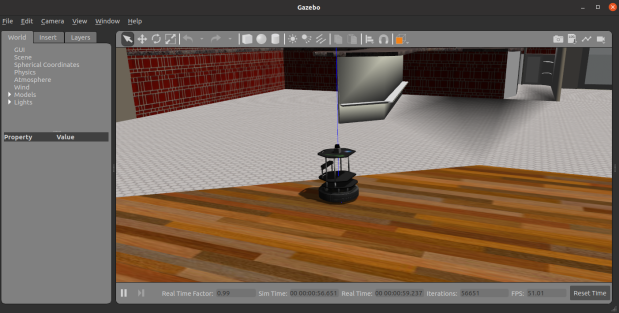
\includegraphics[width=10cm]{imagenes/cap3/simulacion-gazebo.png}
  \end{center}
  \caption{Simulador Gazebo (demostración)}
  \label{fig:simulador_gazebo}
\end{figure}\

¿Cuál ha sido la utilidad de Gazebo en este proyecto? Incorporar un escenario proporcionado por AWS que simula un hospital e integrar el robot simulado Turtlebot2 (sensores incluidos) adaptado para ROS 2 Foxy. El nuevo ejercicio Follow Person simulado hace uso de dicho simulador. La versión del simulador utilizada ha sido \textit{Gazebo 11}.\\




\section{Modelado de robots con URDF y Xacro}
\label{sec:modelado_urdf_xacro}

% -- SUBECCION URDF
% -----------------
\subsection{URDF}
\label{subsec:urdf}

URDF\footnote{\textbf{urdf url:} \url{http://wiki.ros.org/urdf}}  \textit{United Robotics Description Format} es un lenguaje de marcado que usa la gramática de XML para describir robots (eslabones y uniones de eslabones) y sensores (cámaras, láser y muchos otros sensores). Se utiliza tanto para robots reales como simulados.\\

Por lo general el robot se divide en eslabones (\textit{links}) y uniones entre eslabones (\textit{joints}), de manera que se forma un árbol jerárquico de transformadas (TFs) desde un eslabón principal (\textit{root}) hasta los eslabones terminales (\textit{camera\_link}, \textit{laser\_link}, \textit{effector1}, ...).\\

Para definir un \textit{link} hay que proporcionar un modelo visual, un modelo de colisión y un modelo inercial (similar a los videojuegos) [\ref{cod:estructura_urdf}]. Después definimos un \textit{joint} que une el eslabón que hemos definido con otro mediante relación jerárquica de padre e hijo.\\

\begin{code}[H]
\begin{lstlisting}
<?xml version="1.0"?>
<robot name="turtlebot">
	<link name="base">
		<visual>
			...
		</visual>
		<collision>
			...
		</collosion>
		<inertial>
			...
		</inertial>
	</link>
</robot>
\end{lstlisting}
\caption[Estructura URDF de la definicion de un link]{Estructura URDF de la definición de un link}
\label{cod:estructura_urdf}
\end{code}

¿Cuál ha sido la utilidad de URDF en este proyecto? Crear el modelo Turtlebot2 simulado para ROS Foxy. En la Figura \ref{fig:modelo_turtlebot2_simulado} podemos ver el resultado. Veremos más en el capítulo \ref{cap:capitulo4} que tratará del proceso de creación del modelo.
\begin{figure} [H]
  \begin{center}
    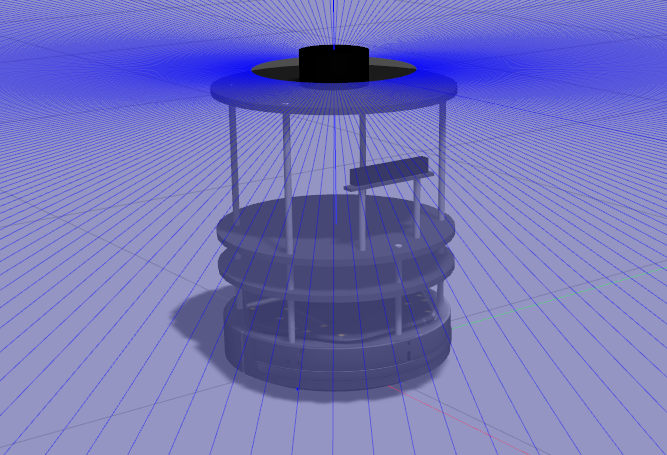
\includegraphics[width=10cm]{imagenes/cap3/turtlebot2-sim.png}
  \end{center}
  \caption{Modelo Turtlebot2 simulado (definido mediante URDF)}
  \label{fig:modelo_turtlebot2_simulado}
\end{figure}\




% -- SECCION XACRO
% ------------------
\subsection{Xacro}
\label{subsec:xacro}

Xacro\footnote{\textbf{Xacro url}: \url{http://wiki.ros.org/xacro}} (XML Macros) es un lenguaje XML diseñado para crear macros \footnote{\textbf{macro}: plantilla que define un patrón} en URDF. Con Xacro conseguimos diseños URDF mucho más legibles y sencillos. De esta manera podemos estructurar el diseño de un robot en componentes más pequeños y repetitivos. Por ejemplo: para el diseño del robot Turtlebot2 creamos una macro que se pueda aplicar a todos las barras verticales que sujetan la estructura del robot.\\

Una vez que tenemos nuestro diseño en Xacro, podemos exportarlo a URDF mediante el paquete de ROS denominado \textit{Xacro}. Su comportamiento es semejante al preprocesador de los lenguajes de programación como C: la macro la sustituye por el código URDF deseado teniendo en cuenta el valor de la variables que haya definido el programador.\\

¿Cuál ha sido la utilidad de Xacro en este proyecto? Diseñar un diseño sencillo y flexible del robot Turtlebot2. En el capítulo \ref{cap:capitulo4} mostraremos mejor la utilidad de Xacro aplicado a nuestro modelo.\\



\section{Tecnologías de frontend}
\label{sec:tecnologias_frontend}

% -- SECCION HTML Y CSS
% -----------------------
\subsection{HTML y CSS}
\label{subsec:html_css}

\textit{HTML (HiperText Markup Language)} es un lenguaje de marcado de tipo XML para el diseño de la estructura de las páginas web. Es un lenguaje que entiende el navegador web y se suele acompañar mediante una hoja de estilos que nos proporciona el lenguaje \textit{CSS (Cascading Style Sheets)} para crear el estilo gráfico de la página web.\\


\begin{code}[H]
\begin{lstlisting}
<p>Esto es un parrafo en HTML</p>
\end{lstlisting}
\begin{lstlisting}
p {
	background-color: #FF0000;
}
\end{lstlisting}
\caption[Ejemplo de HTML y CSS]{Ejemplo de HTML y CSS: Todos los párrafos tienen el fondo rojo}
\label{cod:codigo_urdf}
\end{code}

¿Cuál ha sido la utilidad de HTML y CSS en este proyecto? Diseñar y dar estilo a la plantilla web de los dos nuevos ejercicios de Robotics Academy. El diseño se basó en tomar como referencia las plantillas web de otros ejercicios realizando algunos cambios e incorporando características propias (como por ejemplo, el botón de \textit{teleoperación}).\\




% -- SECCION JavaScript
% -----------------------
\subsection{JavaScript}
\label{subsec:JavaScript}

\textit{JavaScript} es un lenguaje de programación interpretado que destaca por ser utilizado en el lado del cliente, en el \textit{frontend} de una página web que lee el navegador. Con JavaScript podemos crear páginas web dinámicas a través de la definición de eventos que provocan resultados en el \textit{backend} (si tiene) o en la propia estructura HTML. JavaScript puede usarse para multitud de tareas: Websockets, juegos, animaciones, etc.\\

¿Cuál ha sido la utilidad de JavaScript en este proyecto?
En las plantillas web de Robotics Academy se usa JavaScript para comunicar los eventos de la página con el fichero maestro de cada ejercicio que se llama \textit{exercise.py}. La versión de JavaScript utilizada es \textit{ECMAScript 6}



% -- SECCIÓN DOCKER
% -------------------
\section{Docker}
\label{sec:docker}

\textit{Docker}\footnote{\textbf{Docker}: \url{https://www.docker.com/}} es un proyecto de código abierto que nos permite desplegar aplicaciones dentro de contenedores software (máquinas virtuales ligeras que permiten ejecutar múltiples instancias de espacios de usuario) que pueden ejecutar sobre cualquier sistema operativo proporcionando portabilidad al usuario. Por ejemplo, podemos lanzar una aplicación de Linux usando un contenedor Docker, que implementa características del Kernel de Linux, sobre un SO Windows.\\

La creación de imágenes se realiza mediante ficheros \textit{Dockerfile} donde el programador indica los comandos (de Unix) necesarios para la construcción y despliegue de su aplicación. Durante el desarrollo de la imagen se sigue estos pasos:\\

\begin{enumerate}
	\item Importamos una imagen base para empezar. Por ejemplo \textit{FROM osrf/ros:foxy-desktop}
	\item Definimos las variables Dockerfile y de entorno que necesitaremos con \textit{ARG} y \textit{ENV} respectivamente.
	\item Definimos con \textit{RUN} todos los comandos necesarios para la construcción del la imagen \textit{Docker} lanzados desde el directorio de trabajo \textit{WORKDIR}. Con \textit{COPY} copiamos ficheros desde nuestro espacio de usuario al contenedor y con \textit{CMD} indicamos el comando inicial que se ejecutará siempre que lancemos el contenedor.
\end{enumerate}\

¿Cuál ha sido la utilidad de Docker en este proyecto? Cuando Robotics Academy crea una nueva versión construye una imagen Docker con la instalación de todos los repositorios base y de terceros necesarios para la ejecución del entorno web en una distribución de Linux. Gracias a la ejecución de un contenedor el usuario solamente necesita instalar Docker en su SO. Con el comando \textit{docker pull} elige la imagen que quiere descargar y con \textit{docker run} lanza un contenedor para realizar los ejercicios siguiendo sus correspondientes instrucciones. En este proyecto, fue necesario crear una imagen particular en el que funcionara los dos nuevos ejercicios para posteriormente fusionarlos en la nueva imagen oficial RADI 4. La versión de Docker utilizada ha sido 20.10.12\\

En el código [\ref{cod:comando_lanzamiento_docker_unibotics}] vemos qué comando tendría que ejecutar el usuario para lanzar un contenedor con la última imagen de Unibotics y poder interactuar con los ejercicios de la plataforma.\\

\begin{code}[H]
\begin{lstlisting}
$> docker run --rm -it -p 7681:7681 -p 2303:2303 -p 1905:1905 -p 8765:8765 -p 6080:6080 -p 1108:1108 jderobot/robotics-academy:latest ./start_manager.sh
\end{lstlisting}
\caption{Comando de lanzamiento de un contenedor Docker en Unibotics}
\label{cod:comando_lanzamiento_docker_unibotics}
\end{code}\




% -- SECCIÓN DESCRIPCION INFRAESTRUCTURA
% ----------------------------------------

\section{Robotics Academy}
\label{sec:infraestructura_robotics_academy}

\textit{Robotics Academy} \footnote{\textbf{Robotics Academy}: \url{http://jderobot.github.io/RoboticsAcademy/}} es una plataforma web que proporciona una colección de ejercicios de Robótica. Para su ejecución usamos unos contenedores \textit{Docker} [\ref{sec:docker}]  (imagen RADI) que lanza un servidor local (Django) proporcionando todos los ejercicios (las dependencias quedan resueltas) y permitiendo al usuario programar sus soluciones a través del navegador.\\

Por lo general, el usuario dispone en cada ejercicio de un editor de texto, una ventana al simulador de Gazebo y un terminal para depurar su programa. Además, dentro del RADI se lanzan distintos nodos de ROS o incluso el simulador dependiendo del ejercicio. La encapsulación proporcionada hace creer al usuario que todo el procesamiento ocurre en el navegador mientras que en realidad es en el contenedor. El funcionamiento y protocolo de comunicación queda reflejado en la siguiente Figura [\ref{fig:arquitectura_robotics_academy}]:\\

\begin{figure} [H]
  \begin{center}
    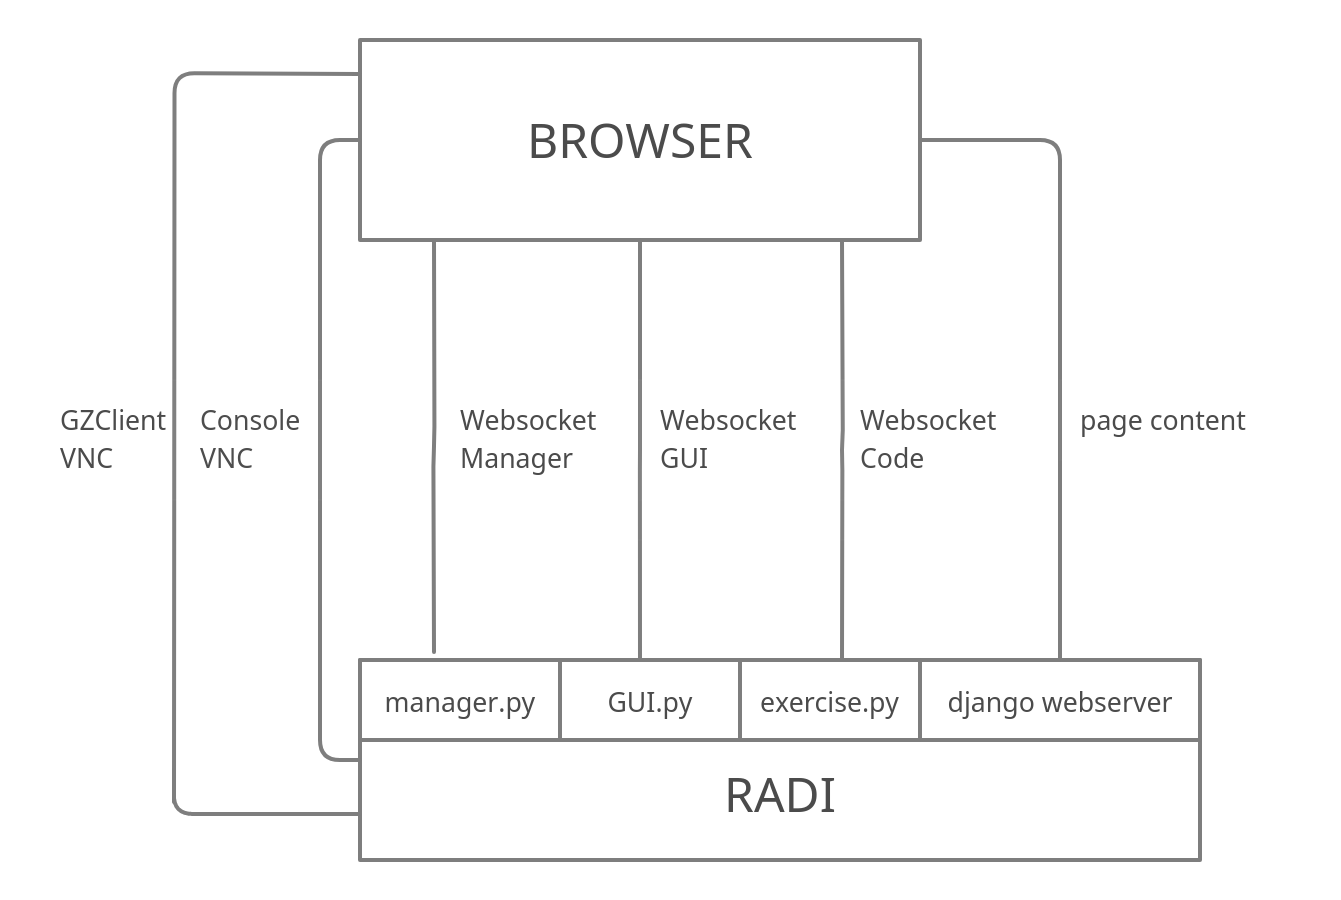
\includegraphics[width=10cm]{imagenes/cap3/robotics_academy_architecture.png}
  \end{center}
  \caption{Arquitectura de Robotics Academy}
  \label{fig:arquitectura_robotics_academy}
\end{figure}\

Cuando lanzamos el contenedor, se ejecuta un servidor \textit{Django} local (usa HTTP) proporcionando los ficheros web (html, css, y js) del menú de inicio; y un fichero de control y administración llamado \textit{manager.py}. El \textit{manager.py} se encarga de controlar la apertura, comunicación y cierre con el ejercicio que solicita el usuario a través \textit{WebSocket Manager} con el navegador. Cada ejercicio implementa una plantilla web específica y un fichero maestro llamado \textit{exercise.py} que se comunica tanto con el \textit{manager.py} como con el navegador. Este fichero proporciona la comunicación con el cerebro del robot mediante el \textit{WebSocket Code} pudiendo de esta manera interactuar con el robot a través de la API de los módulos HAL y GUI. La API de HAL interactúa directamente con los nodos de ROS que cada ejercicio lanza de manera independiente. La visualización de los datos del Robot sobre la plantilla web (como las cámaras) se realiza a través del \textit{WebSocket GUI} que proporciona el fichero \textit{GUI.py}. Por último, para la visualización del simulador y del terminal en el propio navegador se emplean dos conexiones VNC.\\

En la siguiente Figura \ref{fig:infraestructura_robotics_academy} resumimos a modo general la conexión existente entre el navegador y la aplicación de ROS.

\begin{figure} [H]
  \begin{center}
    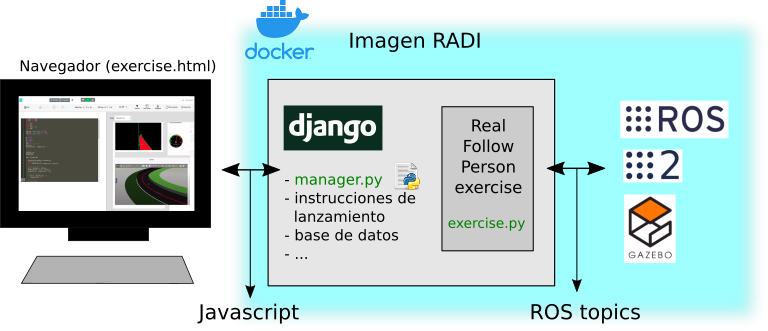
\includegraphics[width=15cm]{imagenes/cap3/esquema-robotics-academy.png}
  \end{center}
  \caption{Arquitectura de Robotics Academy (II)}
  \label{fig:infraestructura_robotics_academy}
\end{figure}\

Actualmente, Robotics Academy dispone de dos ramas de desarrollo: una rama principal que proporciona ejercicios con \textit{ROS Noetic}, y una rama secundaria (en versión beta) que usa \textit{ROS Foxy}. Los dos ejercicios de este TFG han sido incluidos en esta última rama. 


% -- SECCION Turtlebot2
\section{Turtlebot2}
\label{sec:turtlebot2}

El laboratorio de Robótica de la ETSIT URJC tiene a su disposición una decena de robots Turtlebot2 para que los alumnos hagan uso de ellos en algunas asignaturas del grado. Este robot móvil, ideal para la enseñanza e investigación en robótica, consta de dos bases principales:\\

\begin{itemize}
	\item Una base inferior denominada \textit{Kobuki}. Es similar a las aspiradoras de limpieza robóticas como Roomba (iRobot). Respecto al hardware presenta tres sensores de contacto (bumpers) para detectar colisiones con el entorno, odometría, leds programables, sensor de caída y un giroscopio entre otros. Alcanza una velocidad lineal máxima de 0.7 m/s y una velocidad angular de 180 deg/s. Además tiene una batería recargable que opera entre 3 y 7 horas y con alta velocidad de recarga. \textit{Kobuki} tiene soporte real tanto en ROS como en ROS2 con una amplia collección de repositorios en Github\footnote{\textbf{Kobuki (Github)}: \url{https://github.com/kobuki-base}}
\begin{figure} [H]
	\begin{center}
	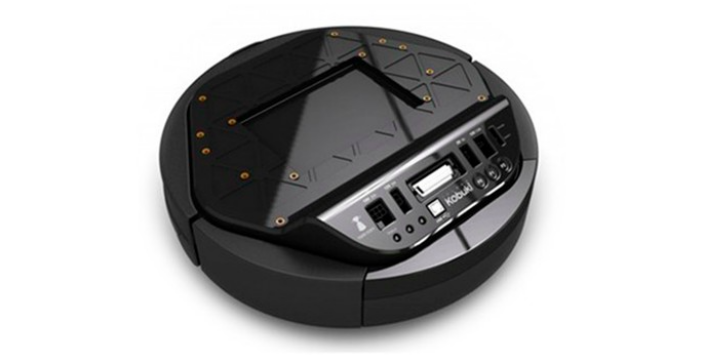
\includegraphics[width=10cm]{imagenes/cap3/base-kobuki.png}
	\end{center}
	\caption[Base Kobuki]{Base \textit{Kobuki}. Imagen obtenida de \cite{kobuki}}
	\label{fig:kobuki_real}
\end{figure}\
	\item Una base superior donde el alumno puede colocar su portatil y conectarse a la base Kobuki mediante USB. Está adaptado para incorporar varios tipos de sensores como cámaras (RGB y RGB-D), láseres e incluso actuadores como un brazo robótico.
\end{itemize}

\begin{figure} [H]
  \begin{center}
    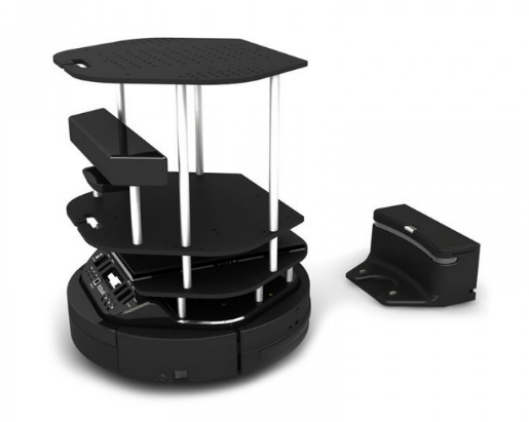
\includegraphics[width=10cm]{imagenes/cap3/turtlebot2-real.png}
  \end{center}
  \caption[Turtlebot2]{Turtlebotd2. Imagen obtenida de \cite{turtlebot2}}
  \label{fig:turtlebot2_real}
\end{figure}\

Para este proyecto hemos necesitado un Turtlebot2 y los siguientes sensores:
\subsection{RPLIDAR A1}
\label{subsec:rplidar_a1}
El láser que hemos usado ha sido un modelo RPLIDAR A1. Se trata de un láser de 360 grados con un alcance de 12 metros y una frecuencia de muestreo de 5.5 Hz. El repositorio de github que hemos utilizado para leer las lecturas del láser se encuentra en este enlace: \url{https://github.com/allenh1/rplidar_ros}\\

\begin{figure} [H]
  \begin{center}
    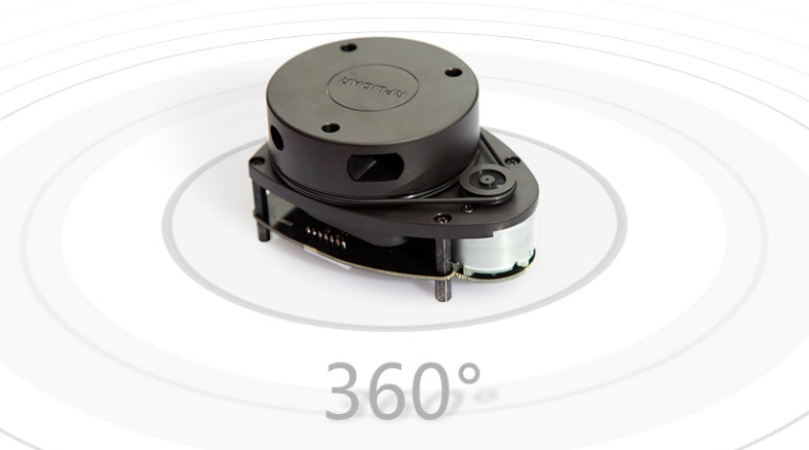
\includegraphics[width=10cm]{imagenes/cap3/rplidar-a1.png}
  \end{center}
  \caption[Láser RPLIDAR A1]{Láser RPLIDAR A1. Imagen obtenida de \cite{rplidar_a1}}
  \label{fig:rplidar_a1}
\end{figure}\

En la Figura [\ref{fig:laser_rvize}] vemos la visualización de las lecturas de un láser con ROS a través de \textit{Rviz}\footnote{\textbf{Rviz}: Visualizador 3D incorporado con ROS}:\\

\begin{figure} [H]
  \begin{center}
    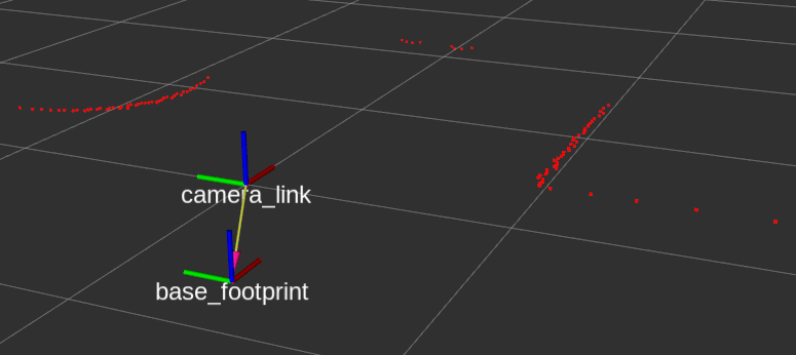
\includegraphics[width=10cm]{imagenes/cap3/laser-rviz.png}
  \end{center}
  \caption[Visualización del láser en Rviz]{Visualización del láser Rviz}
  \label{fig:laser_rviz}
\end{figure}\

\subsection{Cámara Intel Realsense 3d R200}
\label{subsec:intel_realsense_3d}

La cámara usada ha sido una \textit{Intel Realsense 3D R200}. Durante este proyecto hemos probado varias cámaras: Asus XTION PRO Live, Realsense D435 y T265. Debido a la inexistencia de repositorios soportados para ROS Foxy, está fue la cámara candidata. Sin embargo, este modelo no permitia usar la profundidad 3D en ROS, por lo que la utilizamos como una simple cámara RGB. Cualquier cámara que abra dispositivos en /dev/video* (como por ejemplo una webcam) podrá ser utilizado en el ejercicio Real Follow Person. Simplemente tendremos que realizar un mapeo de puertos cuando lancemos el contenedor docker indicado.\\

\begin{figure} [H]
  \begin{center}
    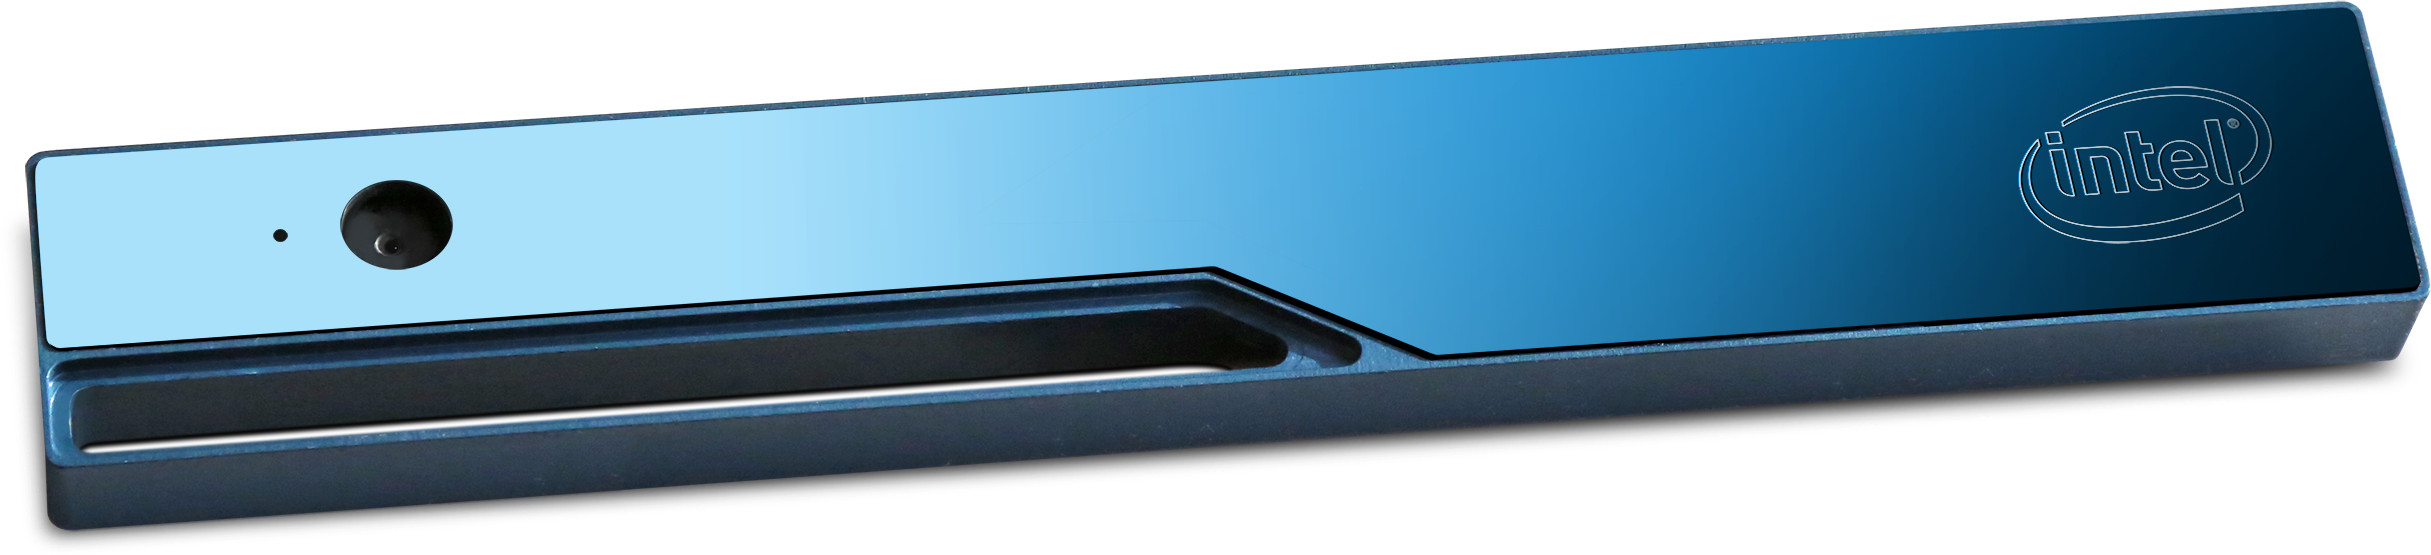
\includegraphics[width=10cm]{imagenes/cap3/r200.jpg}
  \end{center}
  \caption[Cámara Intel Realsense 3D R200]{Cámara Intel Realsense 3D R200. Imagen obtenida de \cite{R200}}
  \label{fig:camara_r200}
\end{figure}\

En la siguiente figura [\ref{fig:camara_rviz}], vemos la visualización del la nube de puntos 3D generada por una cámara RGB-D con ROS a través del visualizador \textit{Rviz}:\\

\begin{figure} [H]
  \begin{center}
    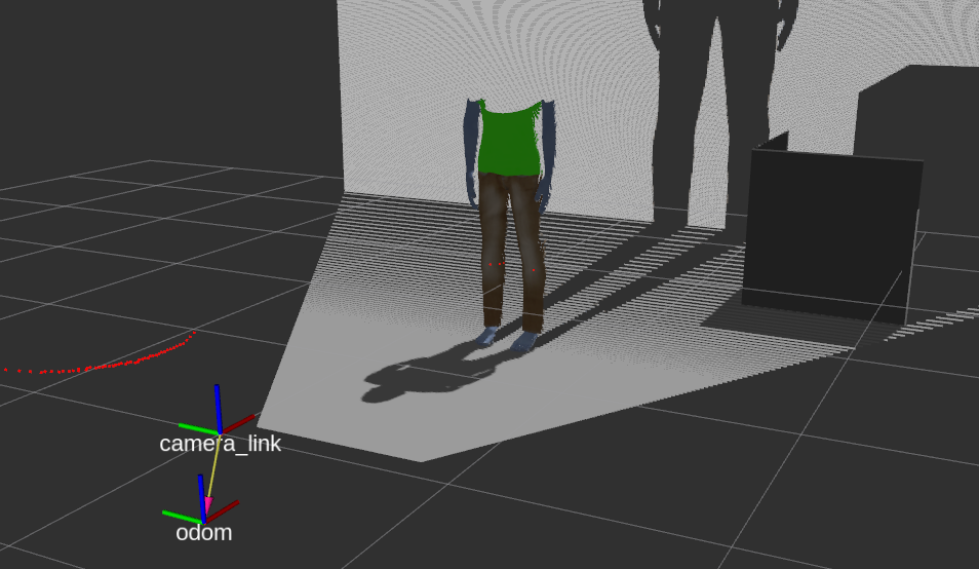
\includegraphics[width=10cm]{imagenes/cap3/camara-rviz.png}
  \end{center}
  \caption[Visualización de una cámara RGBD en Rviz]{Visualización de una cámara RGBD en Rviz}
  \label{fig:camara_rviz}
\end{figure}\


